\documentclass[11pt]{article}
\usepackage[margin=1in]{geometry}
\usepackage{booktabs}
\usepackage{graphicx}
\usepackage{caption}
\usepackage{float}
\usepackage{amsmath}
\usepackage{amssymb}
\graphicspath{{figs/}}
\setlength{\tabcolsep}{5pt}

\title{Phase 2 / Phase 2 Context Analysis}
\author{Howie Zhi-Hong Jian}
\date{\today}

\begin{document}
\maketitle

\section{Regression: Wasserstein-1 on phase\_2\_context}
\begin{table}[H]
\centering
\caption{Regression of Wasserstein-1 on elicitation mode, observed context-incentive prompt-condition cells, and controls (phase\_2\_context). Column (1) is OLS; column (2) is a fractional logit (GLM, Binomial, logit link) with HC1 robust standard errors.}
\label{tab:regression-w1-p2c}
\begin{tabular}{lcc}
\toprule
 & (1) OLS & (2) Fractional Logit \\
\midrule
Chunk & -0.132$^{***}$ & -0.948$^{***}$ \\
 & (0.007) & (0.050) \\
Lab & -0.005 & -0.036 \\
 & (0.012) & (0.081) \\
Lab $\times$ Low & -0.003 & -0.023 \\
 & (0.012) & (0.081) \\
Lab $\times$ High & -0.014 & -0.099 \\
 & (0.012) & (0.085) \\
Classroom & -0.003 & -0.021 \\
 & (0.012) & (0.082) \\
Classroom $\times$ Low & -0.005 & -0.037 \\
 & (0.012) & (0.083) \\
Classroom $\times$ High & 0.014 & 0.095 \\
 & (0.012) & (0.094) \\
Private & -0.006 & -0.039 \\
 & (0.008) & (0.056) \\
Public & -0.008 & -0.059 \\
 & (0.008) & (0.058) \\
Reasoning & -0.010 & -0.073 \\
 & (0.007) & (0.047) \\
Intercept & 0.255$^{***}$ & -1.053$^{***}$ \\
 & (0.011) & (0.071) \\
\midrule N & 672 & 672 \\
R$^2$ & 0.380 & -- \\
Adj.\ R$^2$ & 0.371 & -- \\
Pseudo R$^2$ & -- & 0.382 \\
Log-likelihood & 701.243 & -214.924 \\
\bottomrule
\end{tabular}

\par\smallskip\footnotesize \textit{Notes:} Dependent variable = Wasserstein-1. Standard errors in parentheses (HC1 robust for Fractional Logit). Prompt-condition reference = ``Not Specified / Not Specified'' (no context, no incentive). Privacy Treatment reference = ``Not Specified''. Significance: $^{*}p<0.05$, $^{**}p<0.01$, $^{***}p<0.001$.

\end{table}

\section{Overall Wasserstein-1 Summary (phase\_2)}
\begin{table}[H]
\centering
\caption{Summary statistics of Wasserstein-1 by Mode and ChunkN over phase\_2 behavioral games (Explain Reasoning = True, Extra Flag = []).}
\label{tab:w1-overall-p2}
\begin{tabular}{llrrrrrrrr}
\toprule
Mode & ChunkN & N & avg & std & min & p25 & p50 & p75 & p90 \\
\midrule
Atomic & 1 & 150 & 0.299 & 0.193 & 0.058 & 0.170 & 0.271 & 0.370 & 0.475 \\
Chunk & 10 & 150 & 0.149 & 0.149 & 0.005 & 0.045 & 0.091 & 0.199 & 0.370 \\
Chunk & 20 & 150 & 0.149 & 0.151 & 0.000 & 0.047 & 0.091 & 0.192 & 0.360 \\
Chunk & 25 & 150 & 0.151 & 0.152 & 0.005 & 0.055 & 0.088 & 0.206 & 0.369 \\
Chunk & 50 & 149 & 0.150 & 0.145 & 0.005 & 0.065 & 0.095 & 0.188 & 0.364 \\
Chunk & 100 & 150 & 0.153 & 0.141 & 0.005 & 0.065 & 0.096 & 0.194 & 0.398 \\
\bottomrule
\end{tabular}

\end{table}

\section{Explain Reasoning On vs.\ Off (phase\_2)}
\begin{table}[H]
\centering
\caption{Wasserstein-1 with Explain Reasoning on vs.\ off, restricted to Gemini-3 Flash and Qwen3-235 over ChunkN $\in \{1, 10, 20, 25\}$.}
\label{tab:w1-reasoning-p2}
\begin{tabular}{lllrrrr}
\toprule
Mode & ChunkN & \begin{tabular}[c]{@{}l@{}}Explain\\Reasoning\end{tabular} & N & avg & std & p50 \\
\midrule
Atomic & 1 & False & 30 & 0.343 & 0.228 & 0.358 \\
Atomic & 1 & True & 30 & 0.328 & 0.178 & 0.356 \\
Chunk & 10 & False & 30 & 0.166 & 0.192 & 0.084 \\
Chunk & 10 & True & 30 & 0.153 & 0.149 & 0.106 \\
Chunk & 20 & False & 30 & 0.177 & 0.199 & 0.100 \\
Chunk & 20 & True & 30 & 0.151 & 0.141 & 0.094 \\
Chunk & 25 & False & 30 & 0.183 & 0.203 & 0.104 \\
Chunk & 25 & True & 30 & 0.164 & 0.165 & 0.102 \\
\bottomrule
\end{tabular}

\end{table}

\section{Explain Reasoning On vs.\ Off -- Large Chunks (phase\_2)}
\begin{table}[H]
\centering
\caption{Wasserstein-1 with Explain Reasoning on vs.\ off on phase\_2 behavioral games for ChunkN $\in \{50, 100\}$, grouped by ChunkN, Explain Reasoning, SplitN, and Reasoning Mode (chunk elicitation only). All LLM models included.}
\label{tab:w1-reasoning-large-chunks-p2}
\normalsize
\setlength{\tabcolsep}{3pt}
\begin{tabular}{llllrrrr}
\toprule
ChunkN & \begin{tabular}[c]{@{}l@{}}Explain\\Reasoning\end{tabular} & SplitN & \begin{tabular}[c]{@{}l@{}}Reasoning\\Mode\end{tabular} & N & avg & std & p50 \\
\midrule
50 & False & -- & basic & 150 & 0.167 & 0.180 & 0.096 \\
50 & True & 25 & split & 149 & 0.150 & 0.145 & 0.095 \\
100 & False & -- & basic & 150 & 0.188 & 0.187 & 0.129 \\
100 & True & 25 & split & 150 & 0.153 & 0.141 & 0.096 \\
\bottomrule
\end{tabular}

\end{table}

\section{Wasserstein-1 Summary by Mode (Ground-truth Games)}
\begin{table}[H]
\centering
\caption{Wasserstein-1 summary statistics over the four ground-truth games (TicTacToe Logic L2, TicTacToe Logic, Arithmetic Verification, Trivial Dominance), phase\_2, ChunkN $\in \{1, 10\}$, Explain Reasoning = True.}
\label{tab:gt-summary-mode}
\begin{tabular}{lrrrrrrrrr}
\toprule
Mode & N & \begin{tabular}[c]{@{}l@{}}Num of\\W1$>$0\end{tabular} & avg & std & min & p25 & p50 & p75 & p90 \\
\midrule
Atomic & 60 & 5 & 0.004 & 0.021 & 0.000 & 0.000 & 0.000 & 0.000 & 0.000 \\
Chunk & 60 & 13 & 0.021 & 0.058 & 0.000 & 0.000 & 0.000 & 0.000 & 0.072 \\
\bottomrule
\end{tabular}

\end{table}

\section{Ground-truth Non-zero W1 with Error Rates}
\begin{table}[H]
\centering
\caption{Simulations on ground-truth games (Explain Reasoning = True) where Wasserstein-1 $\neq 0$, with the share of decisions misaligned with the ground-truth benchmark (Misaligned \%). Each listed simulation pools $N=100$ decisions.}
\label{tab:gt-errors}
\begin{tabular}{lllrr}
\toprule
Game & Mode & LLM Model & Misaligned \% & Wasserstein-1 \\
\midrule
Arithmetic Verification & Chunk & Grok 4 & 5.0 & 0.001 \\
Arithmetic Verification & Chunk & Grok 4 & 11.0 & 0.002 \\
Arithmetic Verification & Chunk & Grok 4.1 Fast & 3.0 & 0.000 \\
TicTacToe Logic & Chunk & Grok 4 & 16.0 & 0.160 \\
TicTacToe Logic & Chunk & Grok 4 & 22.0 & 0.220 \\
TicTacToe Logic - L2 & Atomic & DeepSeek V3.2 & 16.0 & 0.160 \\
TicTacToe Logic - L2 & Atomic & DeepSeek V3.2 & 1.0 & 0.010 \\
TicTacToe Logic - L2 & Atomic & Gemini 3.1 Pro & 3.0 & 0.030 \\
TicTacToe Logic - L2 & Atomic & Grok 4.1 Fast & 1.0 & 0.010 \\
TicTacToe Logic - L2 & Atomic & Grok 4.1 Fast & 1.0 & 0.010 \\
TicTacToe Logic - L2 & Chunk & Qwen 3 & 1.0 & 0.010 \\
TicTacToe Logic - L2 & Chunk & Grok 4 & 15.0 & 0.150 \\
TicTacToe Logic - L2 & Chunk & Grok 4 & 14.0 & 0.140 \\
TicTacToe Logic - L2 & Chunk & Grok 4.1 Fast & 1.0 & 0.010 \\
Trivial Dominance & Chunk & GPT-5.2 & 6.0 & 0.060 \\
Trivial Dominance & Chunk & GPT-5.2 & 7.0 & 0.065 \\
Trivial Dominance & Chunk & Grok 4 & 20.0 & 0.200 \\
Trivial Dominance & Chunk & Grok 4 & 24.0 & 0.240 \\
\bottomrule
\end{tabular}

\end{table}

\section{Random Number Generation Summary}
\begin{table}[H]
\centering
\caption{Wasserstein-1 summary statistics for Random Number Generation, phase\_2, grouped by Mode, ChunkN, and Temperature, with Extra Flag = [] or small\_experiments\_on\_temperature.}
\label{tab:w1-random-number-generation-p2}
\begin{tabular}{lrrrrrrrrrr}
\toprule
Mode & ChunkN & Temperature & N & avg & std & min & p25 & p50 & p75 & p90 \\
\midrule
Atomic & 1 & 1 & 15 & 0.206 & 0.043 & 0.144 & 0.168 & 0.208 & 0.248 & 0.253 \\
Atomic & 1 & 2 & 11 & 0.194 & 0.056 & 0.090 & 0.143 & 0.211 & 0.238 & 0.249 \\
Chunk & 10 & 1 & 15 & 0.028 & 0.010 & 0.017 & 0.023 & 0.026 & 0.029 & 0.044 \\
\bottomrule
\end{tabular}

\end{table}

\section{Figures}

\begin{figure}[H]
\centering
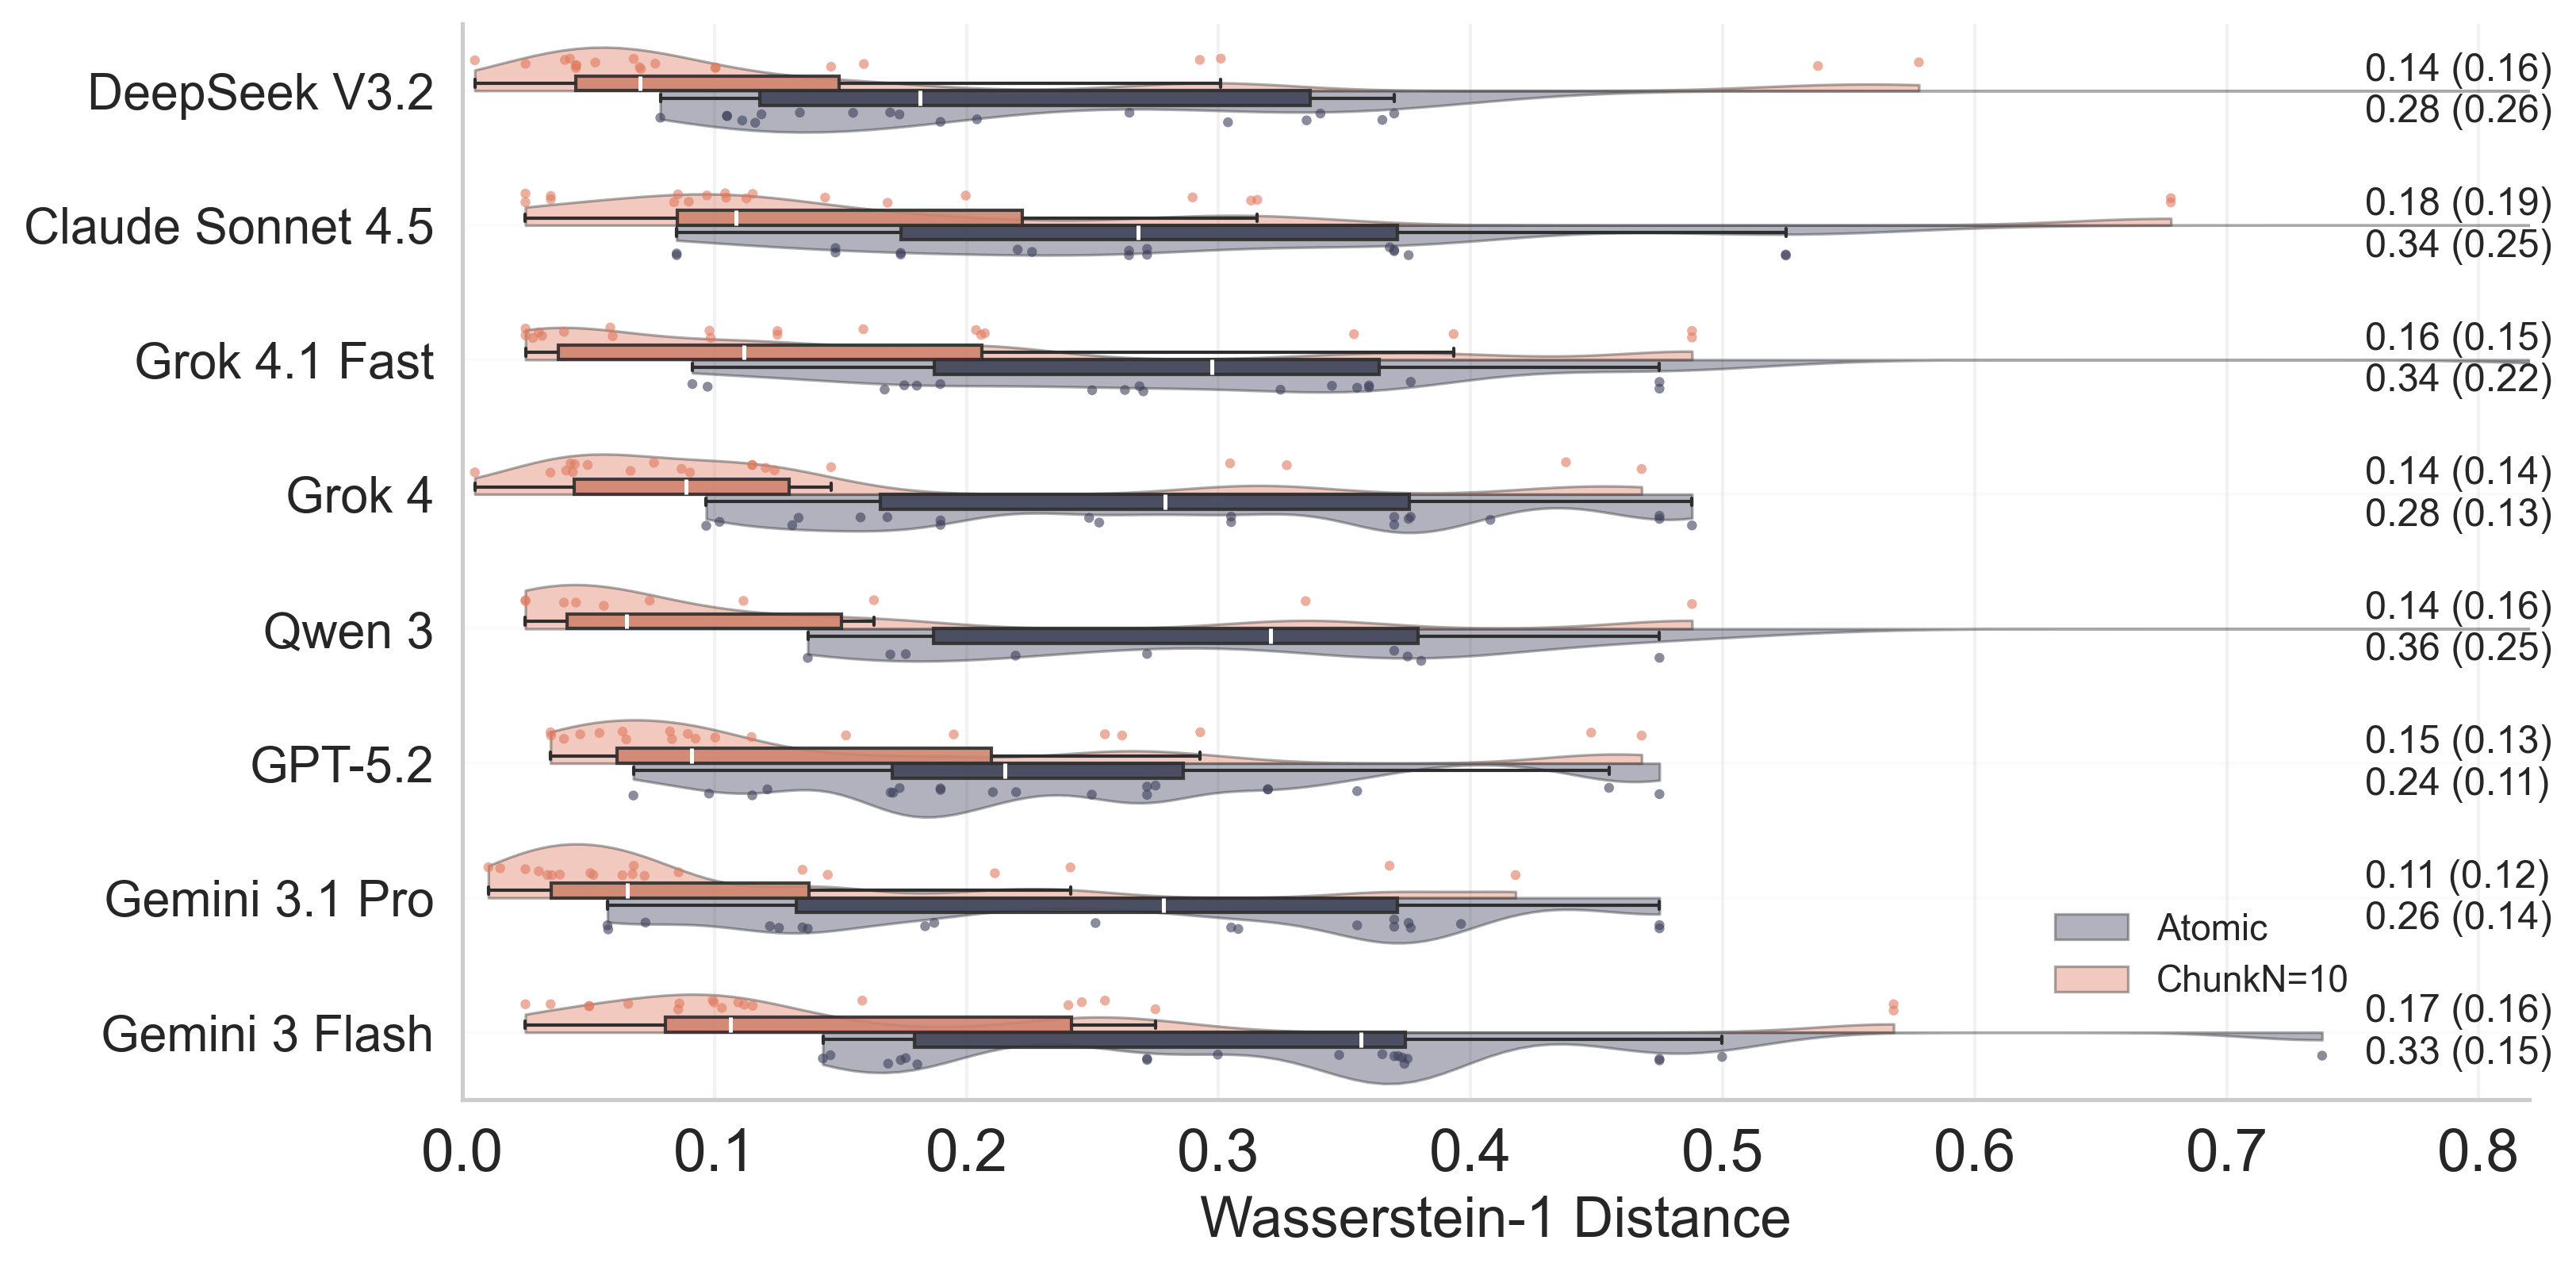
\includegraphics[width=\textwidth]{table2_raincloud_model_performance.png}
\caption{Raincloud of W1 by LLM Model, split by elicitation mode (ChunkN=10 vs.\ Atomic).}
\label{fig:raincloud-model}
\end{figure}

\begin{figure}[H]
\centering
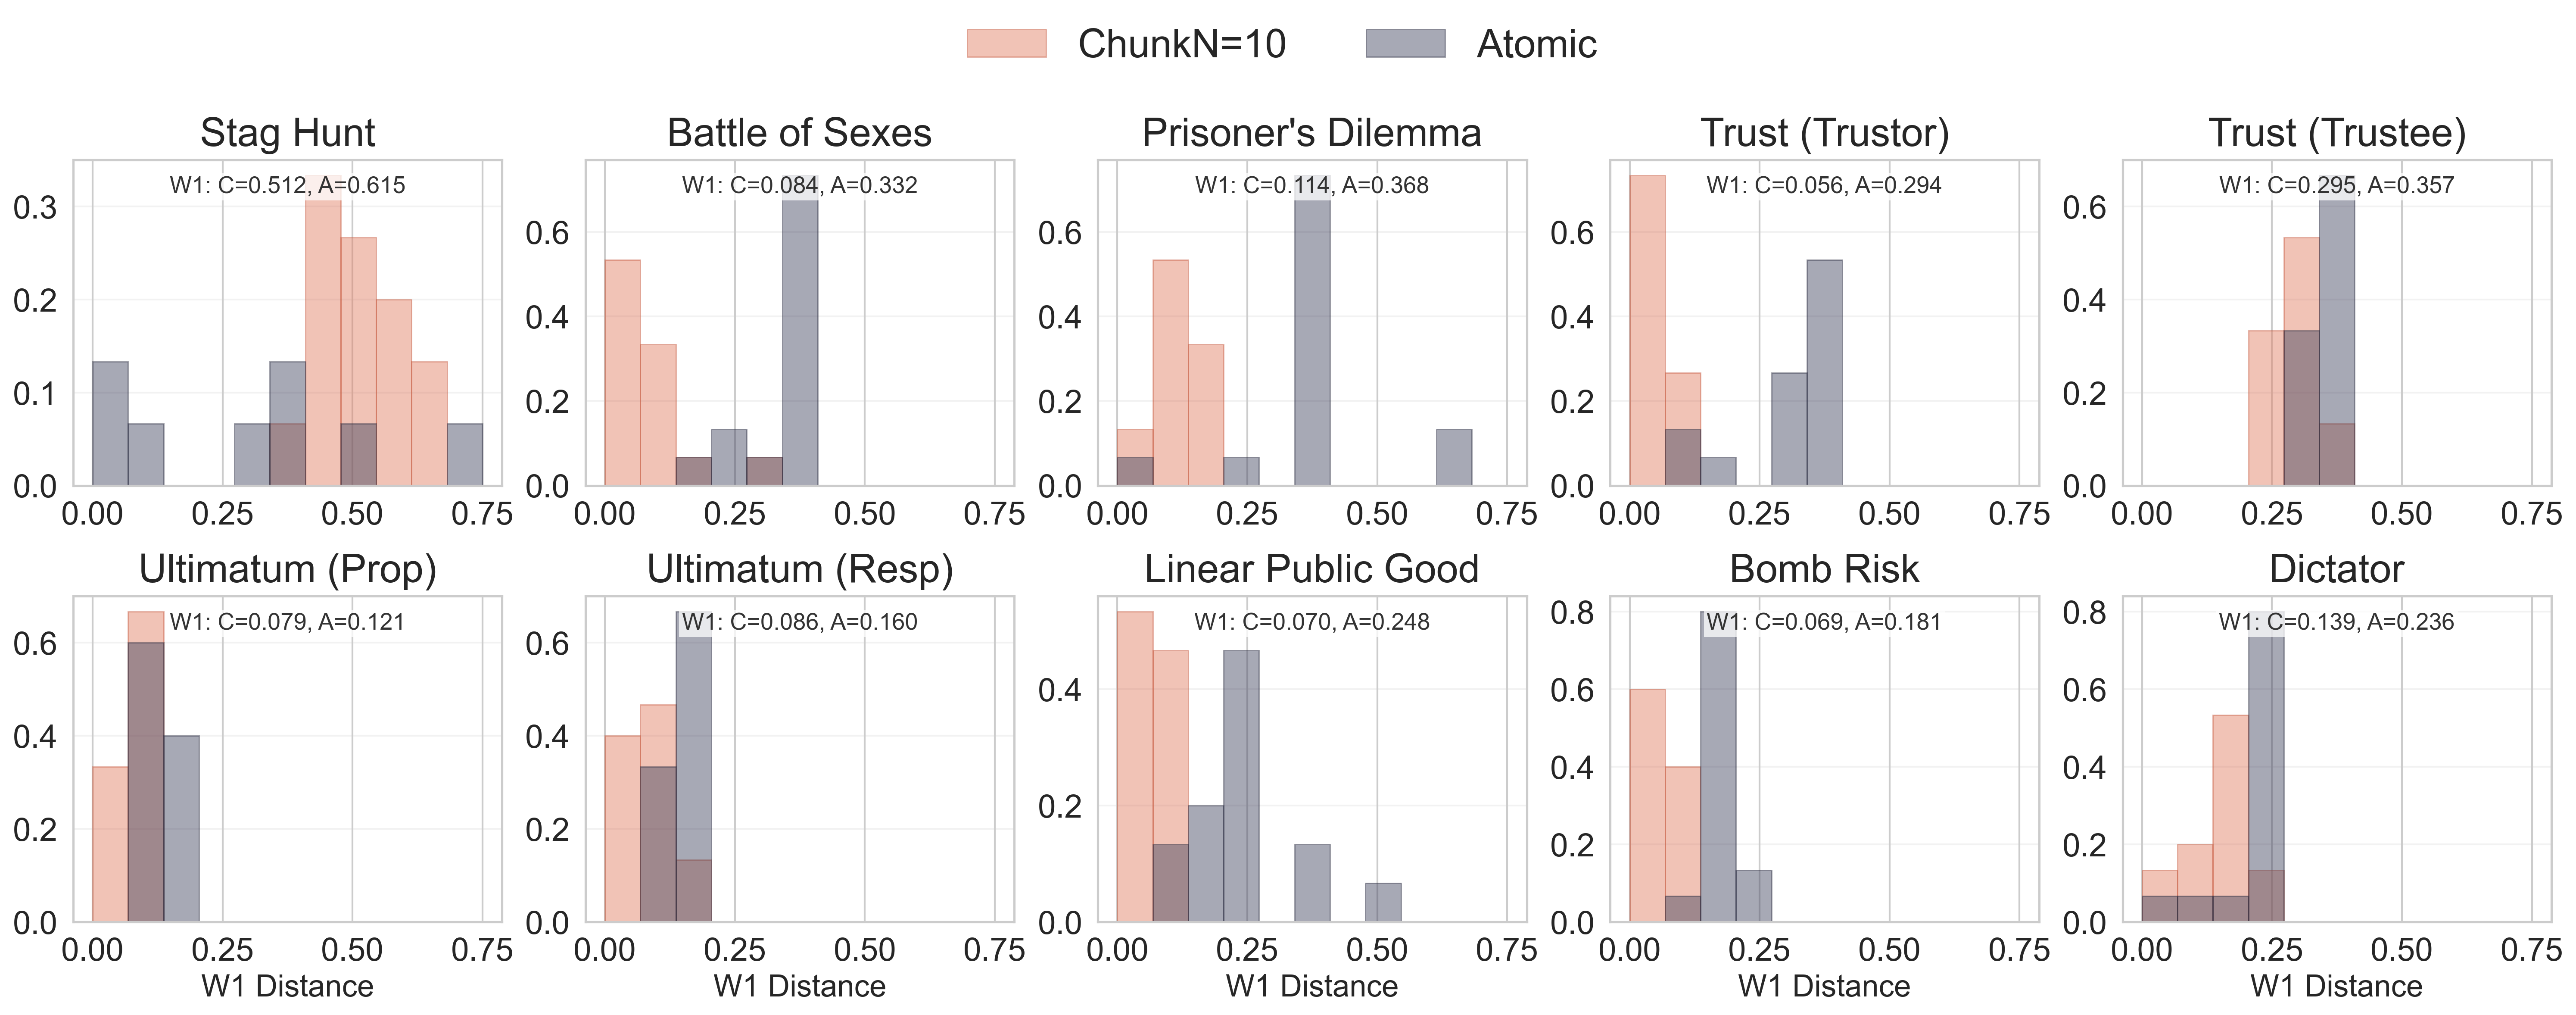
\includegraphics[width=\textwidth]{task1b_w1_by_game.png}
\caption{Distribution of W1 by game, ChunkN=10 vs.\ Atomic.}
\label{fig:w1-by-game}
\end{figure}

\begin{figure}[H]
\centering
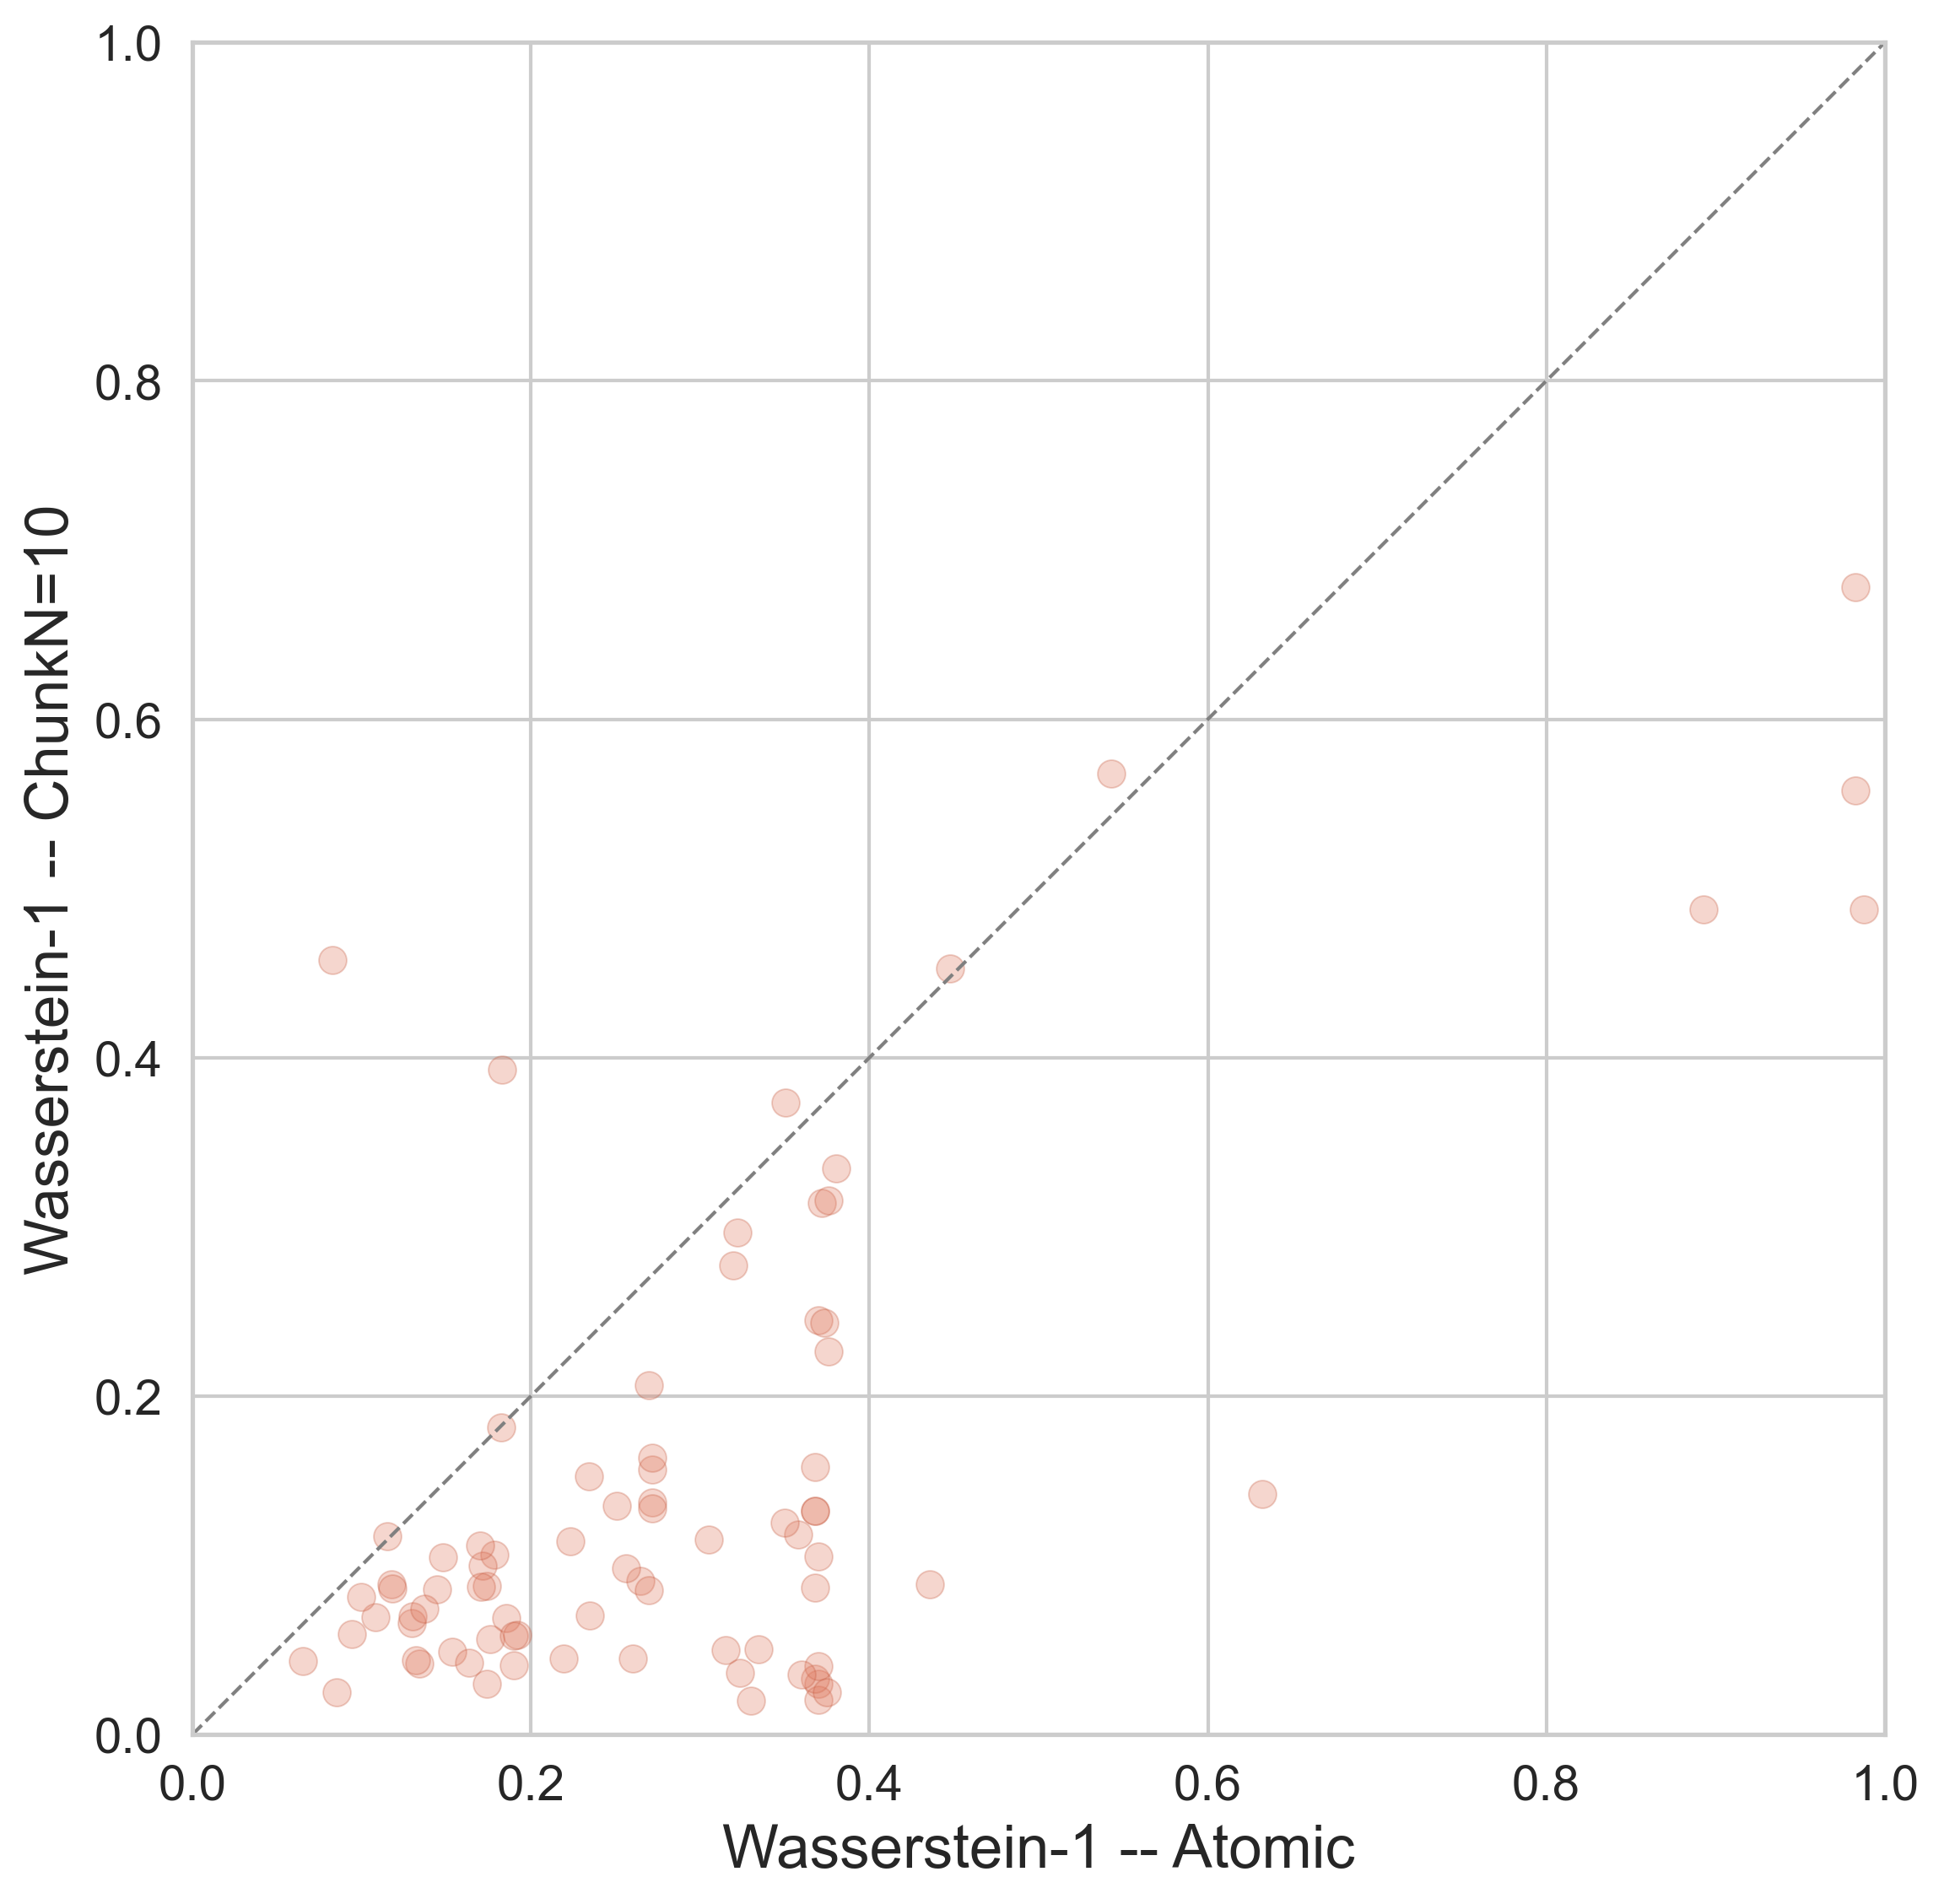
\includegraphics[width=0.7\textwidth]{task1c_atomic_vs_chunk10_scatter.png}
\caption{Atomic vs.\ ChunkN=10 per-(Model, Game) mean Wasserstein-1. Each point is one (LLM Model, Game) pair over the phase\_2 behavioral-game scope; the dashed grey line is the equality reference. Points with $\alpha=0.1$ convey density; points below the line indicate ChunkN=10 reduces W1 relative to Atomic.}
\label{fig:atomic-vs-chunk-scatter}
\end{figure}

\begin{figure}[H]
\centering
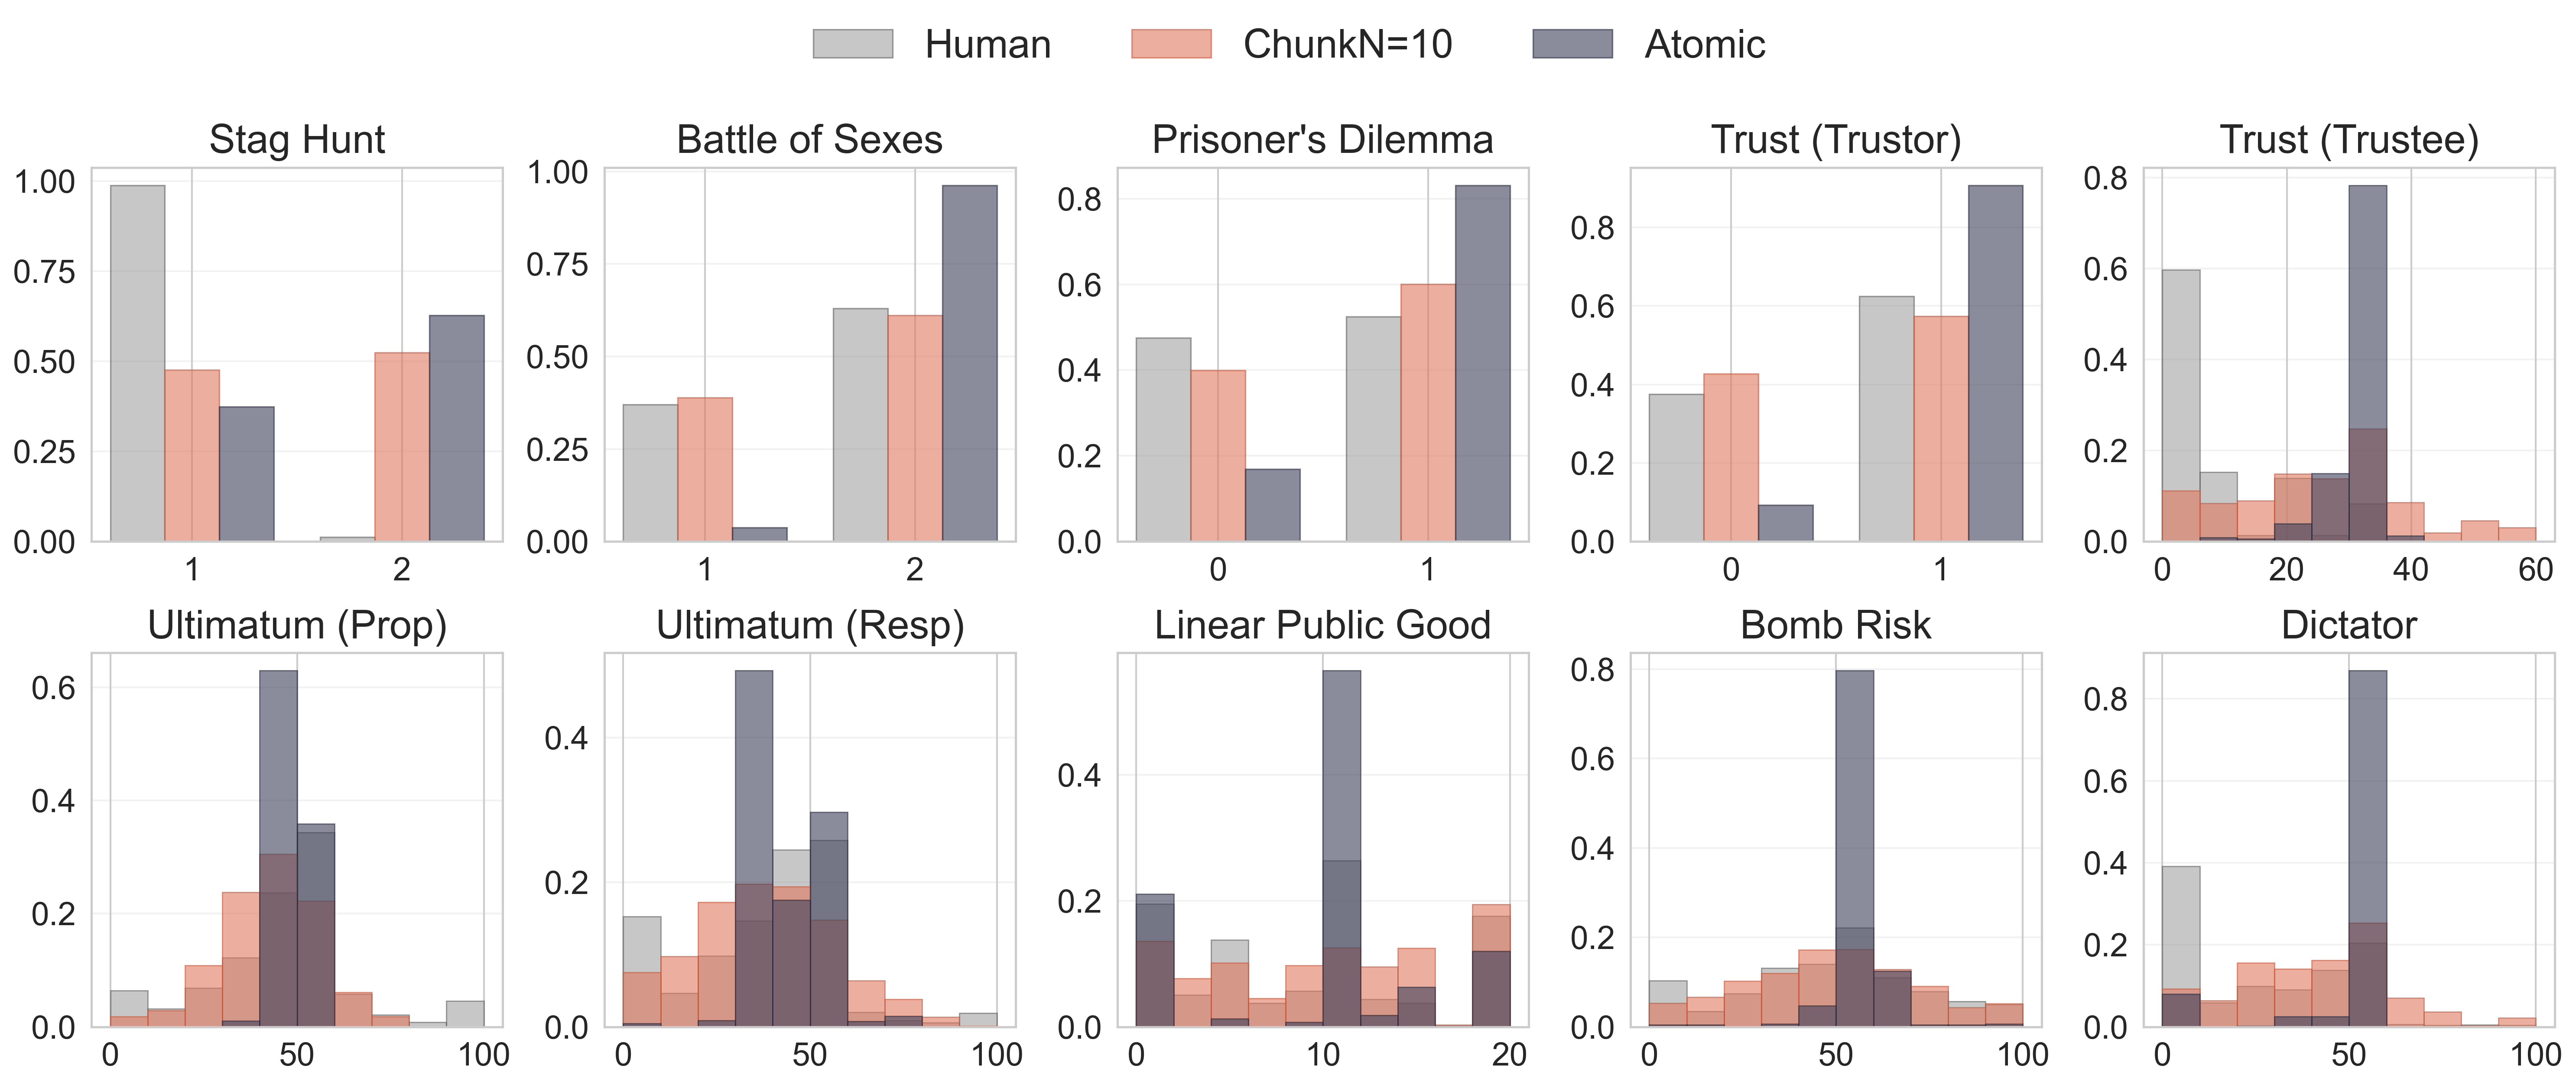
\includegraphics[width=\textwidth]{task2_decision_distributions.png}
\caption{Decision distributions across behavioral games: human benchmark vs.\ ChunkN=10 vs.\ Atomic.}
\label{fig:dist-behavior}
\end{figure}

\begin{figure}[H]
\centering
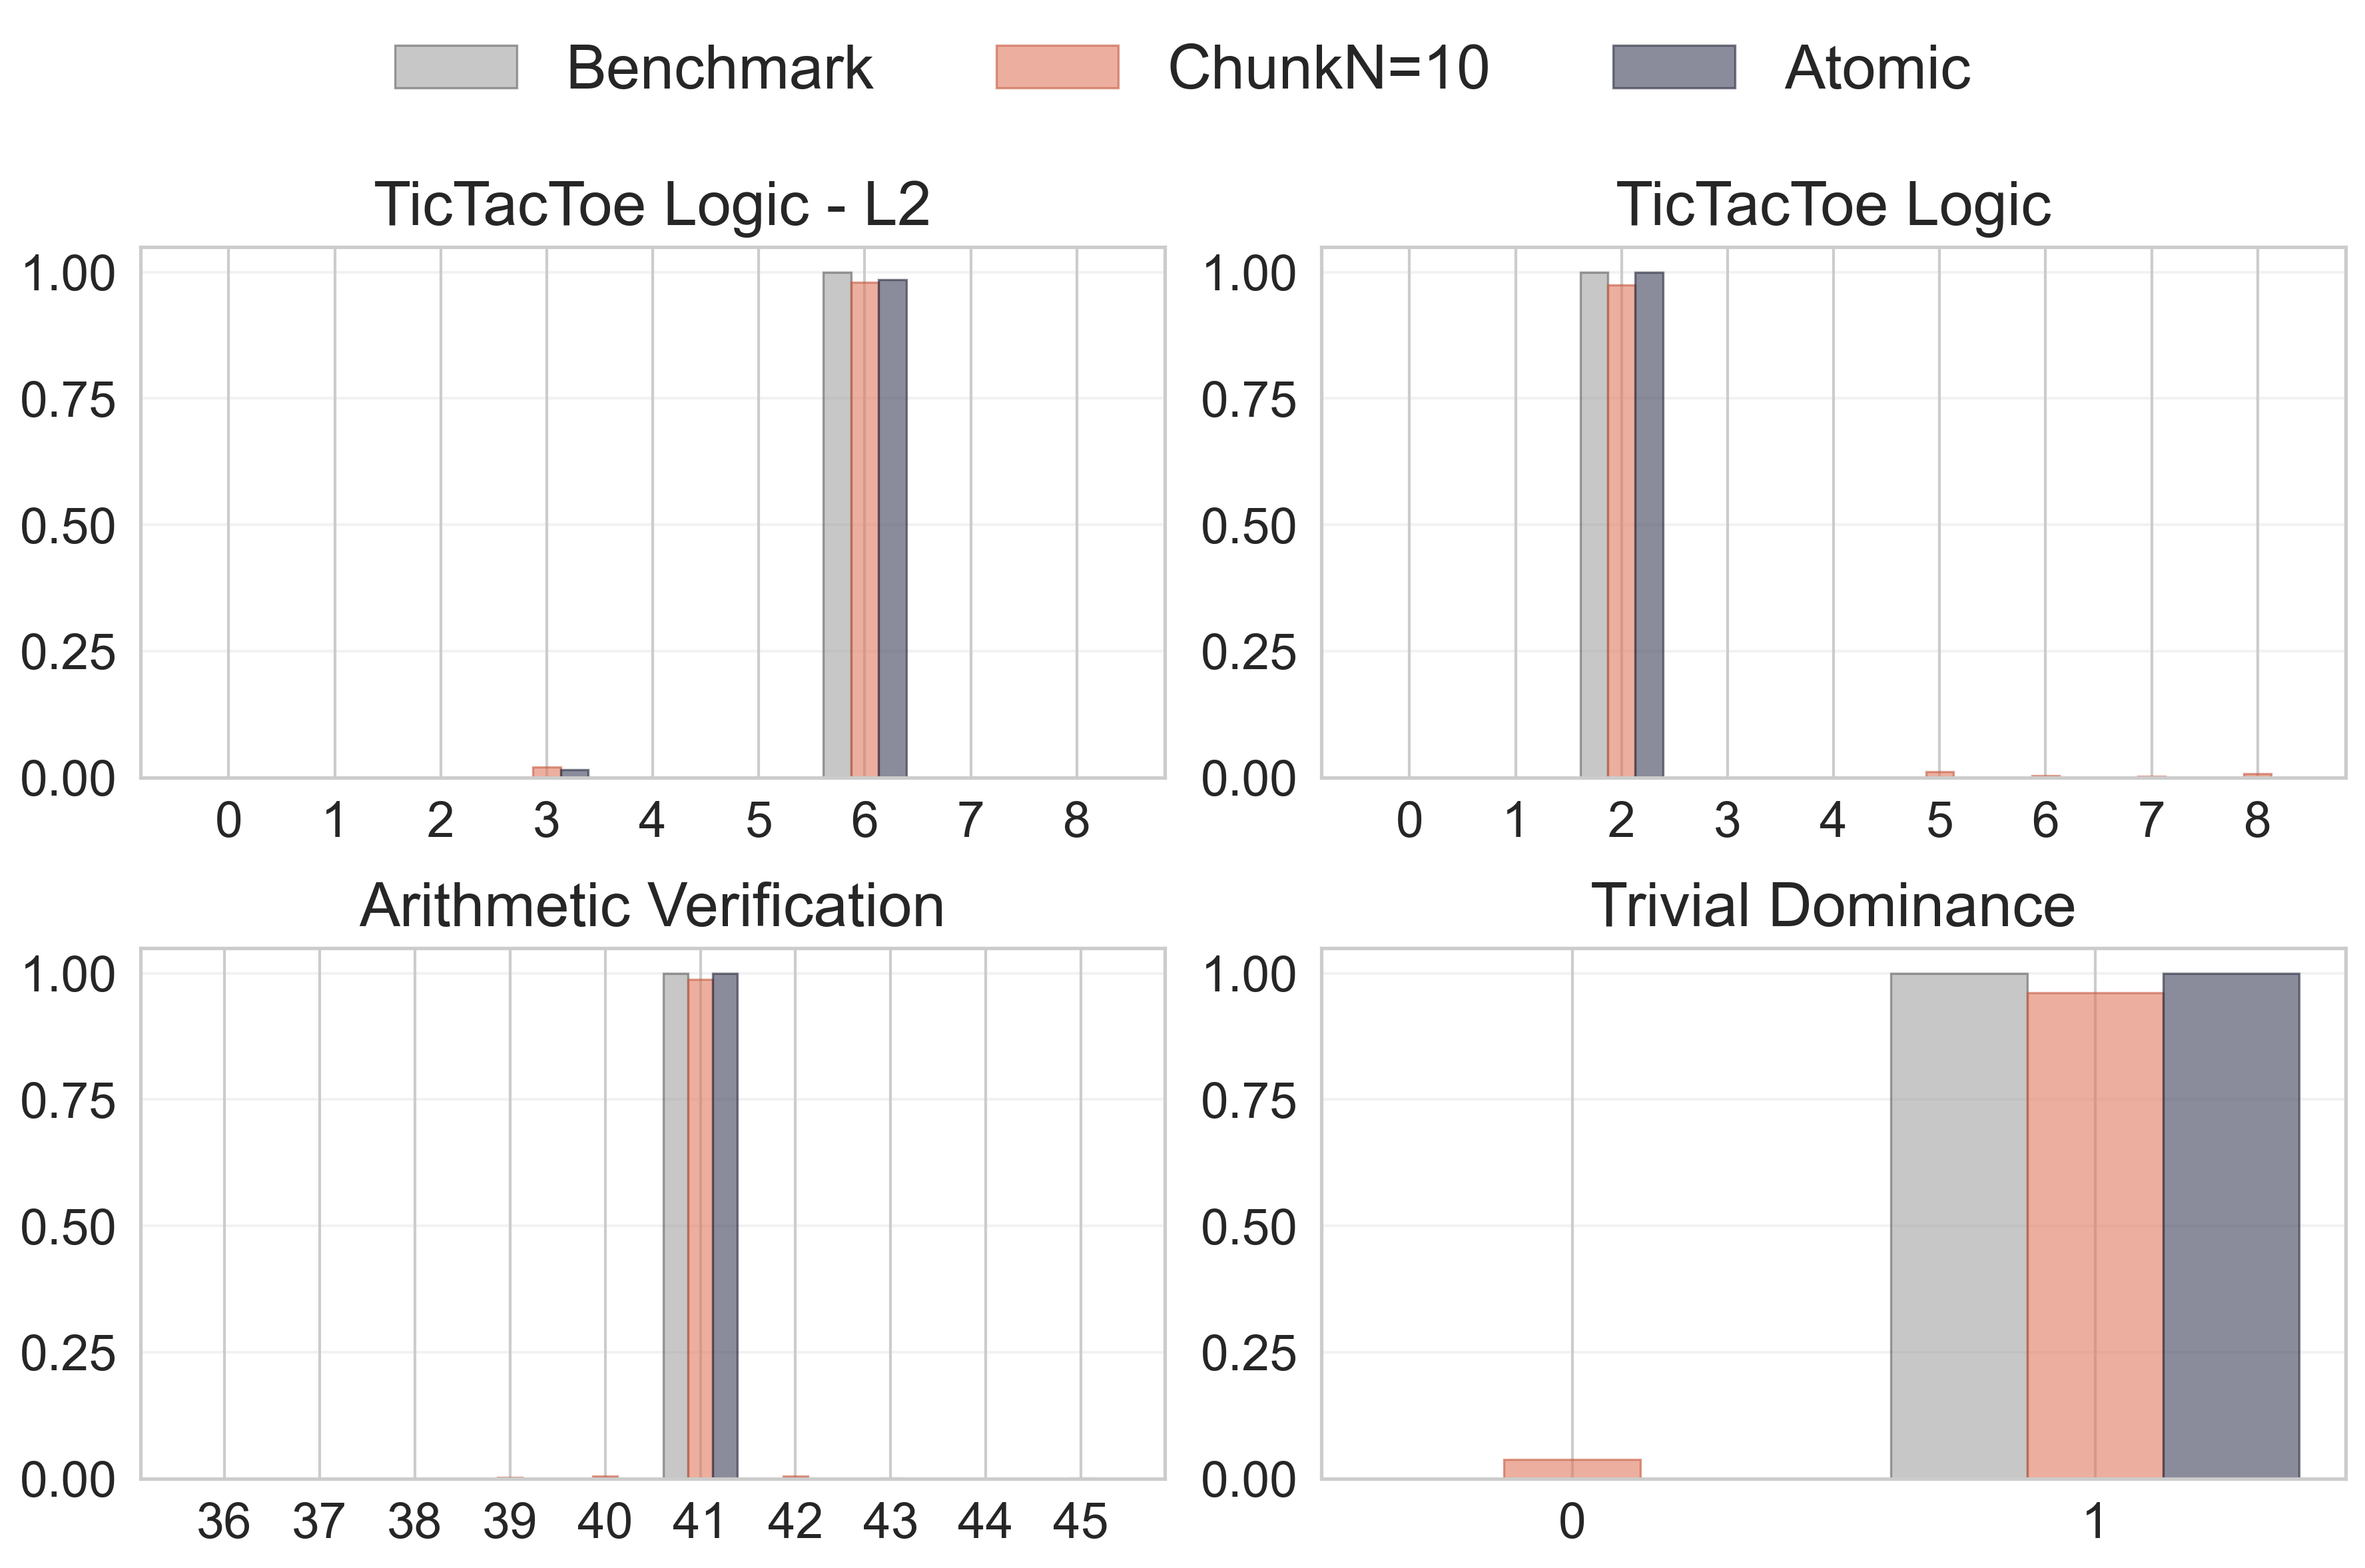
\includegraphics[width=\textwidth]{task2b_ground_truth_decision_distributions.png}
\caption{Decision distributions for ground-truth games: benchmark vs.\ ChunkN=10 vs.\ Atomic.}
\label{fig:dist-groundtruth}
\end{figure}

\section{Within-response Mechanism}

\begin{figure}[H]
\centering
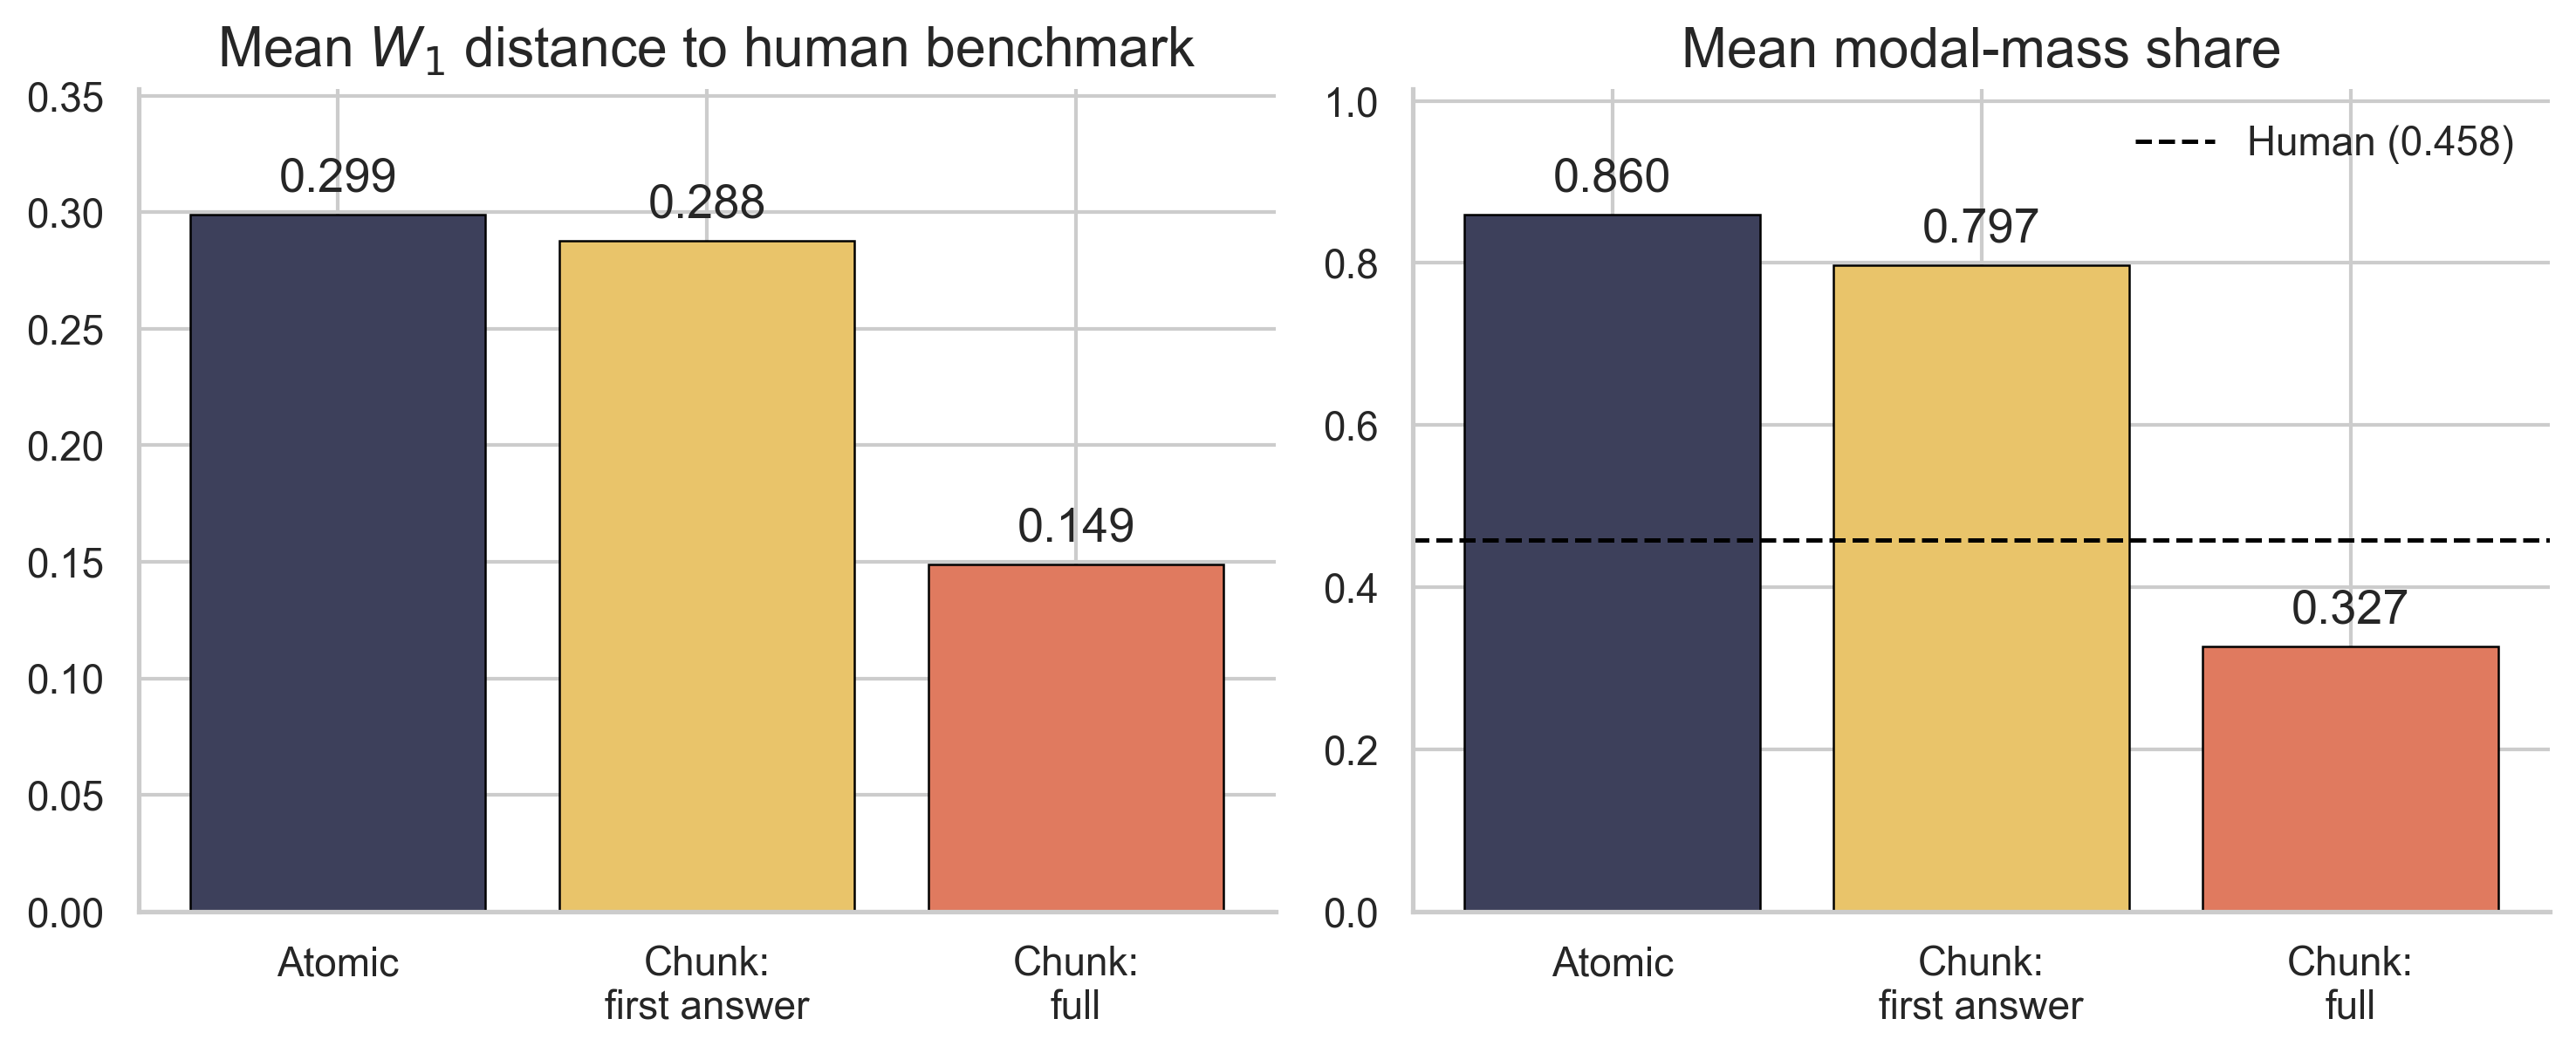
\includegraphics[width=0.95\textwidth]{mechanism_first_answer.png}
\caption{Distance to the human benchmark and modal-mass share for atomic elicitation, the first answer from each chunk call, and the full chunk distribution.}
\label{fig:mech-first-answer}
\end{figure}

\begin{table}[H]
\centering
\caption{Position-wise mechanism results for Answers 1--10.}
\label{tab:mech-position-answer}
\resizebox{\textwidth}{!}{\normalsize
\setlength{\tabcolsep}{3pt}
\begin{tabular}{lcccc}
\toprule
Distribution & $W_1\!\to$ Human & Modal share & $W_1\!\to$ Atomic & $W_1\!\to$ Full \\
\midrule
Atomic & 0.299 & 0.860 & -- & -- \\
Answer 1 & 0.288 & 0.797 & 0.123 & 0.215 \\
Answer 2 & 0.305 & 0.703 & 0.315 & 0.228 \\
Answer 3 & 0.251 & 0.653 & 0.223 & 0.199 \\
Answer 4 & 0.255 & 0.623 & 0.272 & 0.178 \\
Answer 5 & 0.239 & 0.574 & 0.260 & 0.163 \\
Answer 6 & 0.208 & 0.559 & 0.235 & 0.141 \\
Answer 7 & 0.227 & 0.554 & 0.271 & 0.146 \\
Answer 8 & 0.213 & 0.536 & 0.248 & 0.149 \\
Answer 9 & 0.225 & 0.520 & 0.269 & 0.154 \\
Answer 10 & 0.221 & 0.527 & 0.224 & 0.134 \\
Chunk: full & 0.149 & 0.327 & -- & -- \\
Human benchmark & 0.000 & 0.458 & -- & -- \\
\bottomrule
\end{tabular}
}
\end{table}

\begin{figure}[H]
\centering
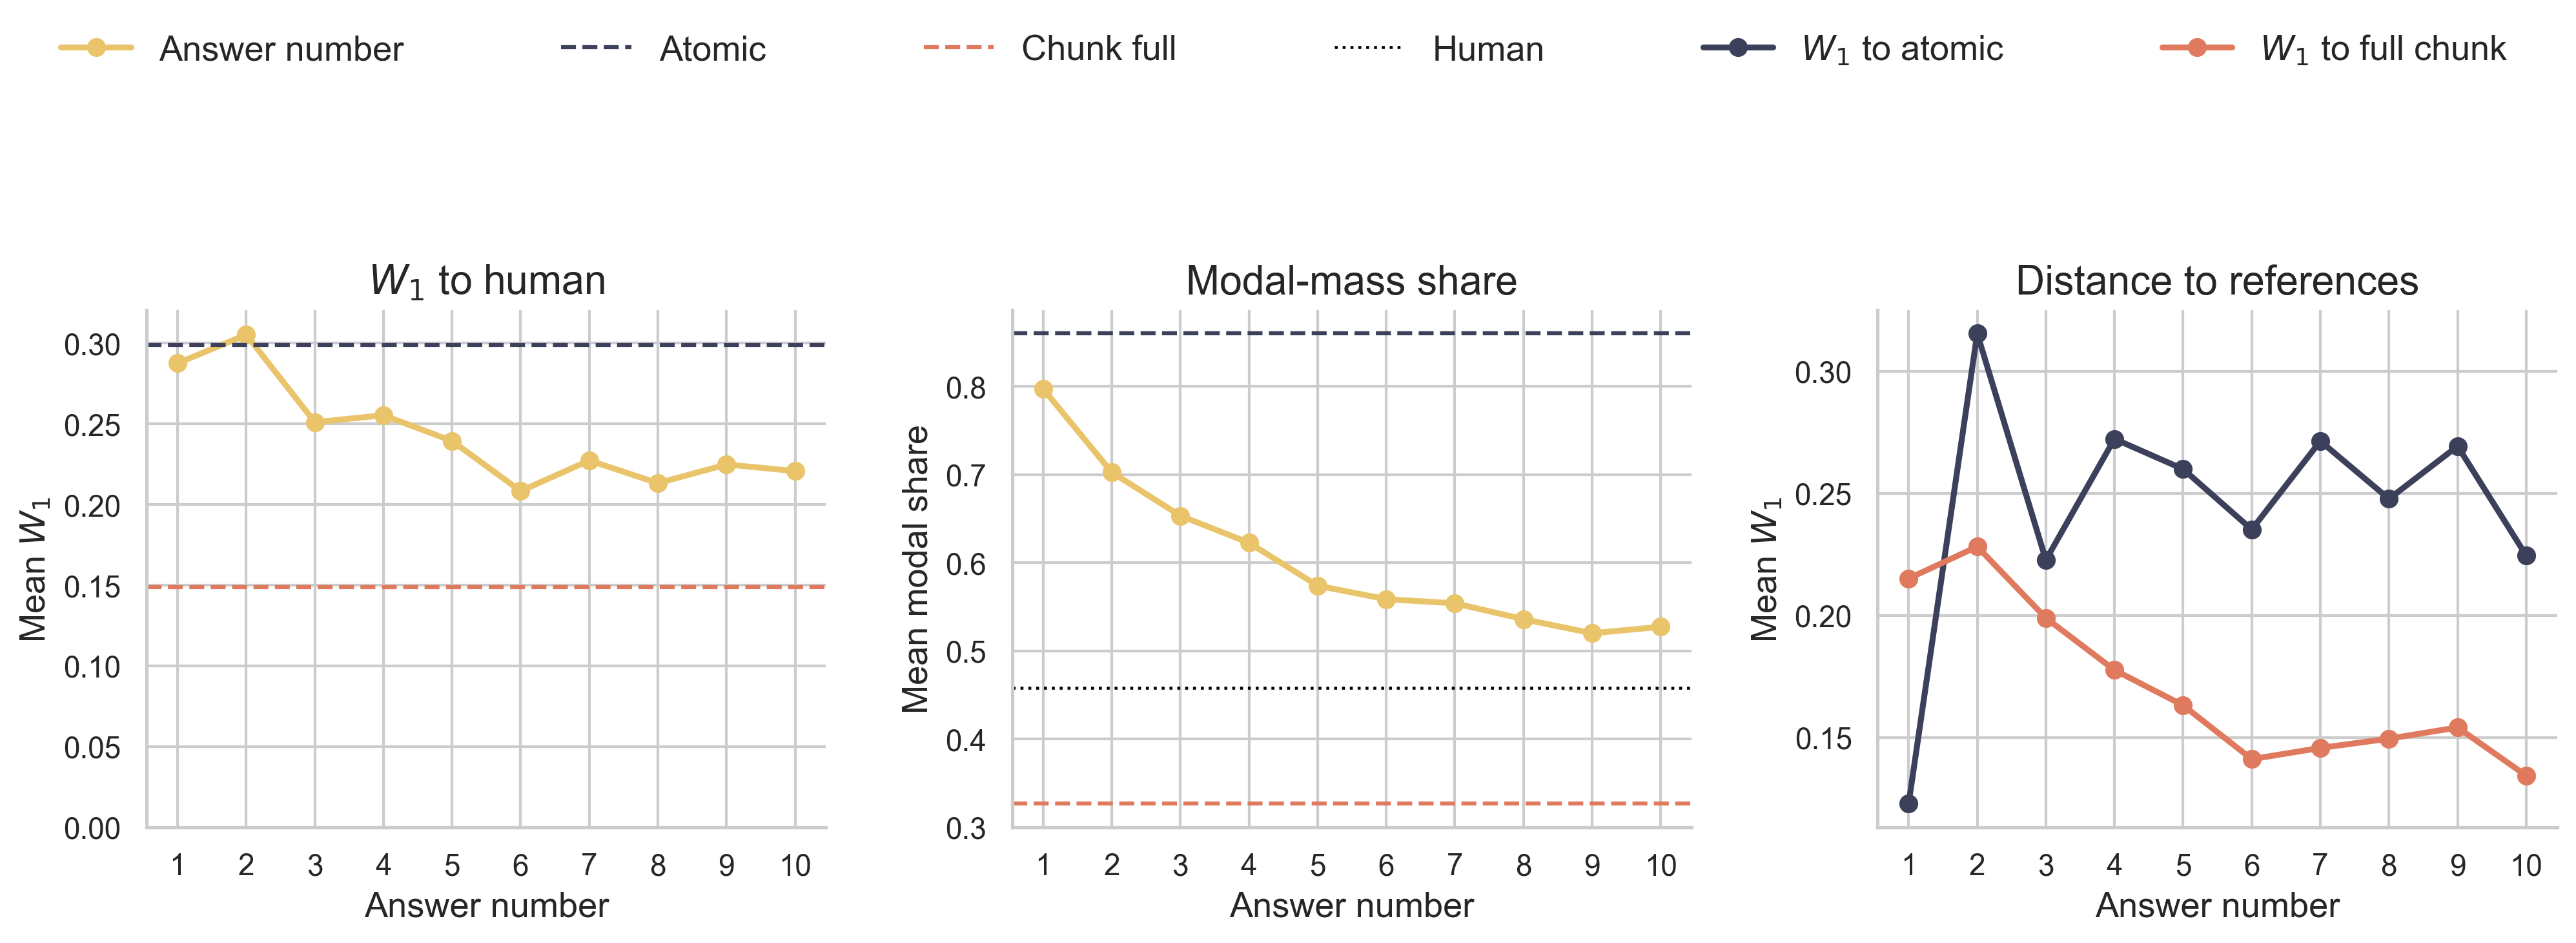
\includegraphics[width=\textwidth]{mechanism_position_answer_w1.png}
\caption{Distance and concentration by answer position within chunked responses.}
\label{fig:mech-position-answer}
\end{figure}

\begin{table}[H]
\centering
\caption{Cumulative mechanism results after pooling the first $k$ answer positions.}
\label{tab:mech-cumulative-answer}
\resizebox{\textwidth}{!}{\begin{tabular}{lrcccc}
\toprule
Distribution & Mean $n$ & $W_1\!\to$ Human & Modal share & $W_1\!\to$ Atomic & $W_1\!\to$ Full \\
\midrule
Atomic & 100 & 0.299 & 0.860 & -- & -- \\
First 1 answer & 10 & 0.288 & 0.797 & 0.123 & 0.215 \\
First 2 answers & 20 & 0.193 & 0.506 & 0.199 & 0.085 \\
First 3 answers & 30 & 0.164 & 0.460 & 0.197 & 0.070 \\
First 4 answers & 40 & 0.160 & 0.401 & 0.212 & 0.041 \\
First 5 answers & 50 & 0.152 & 0.382 & 0.218 & 0.035 \\
First 6 answers & 60 & 0.148 & 0.364 & 0.218 & 0.023 \\
First 7 answers & 70 & 0.151 & 0.350 & 0.224 & 0.022 \\
First 8 answers & 80 & 0.147 & 0.341 & 0.224 & 0.015 \\
First 9 answers & 90 & 0.150 & 0.332 & 0.228 & 0.015 \\
First 10 answers & 100 & 0.149 & 0.327 & 0.226 & 0.000 \\
Human benchmark & -- & 0.000 & 0.458 & -- & -- \\
\bottomrule
\end{tabular}
}
\end{table}

\begin{figure}[H]
\centering
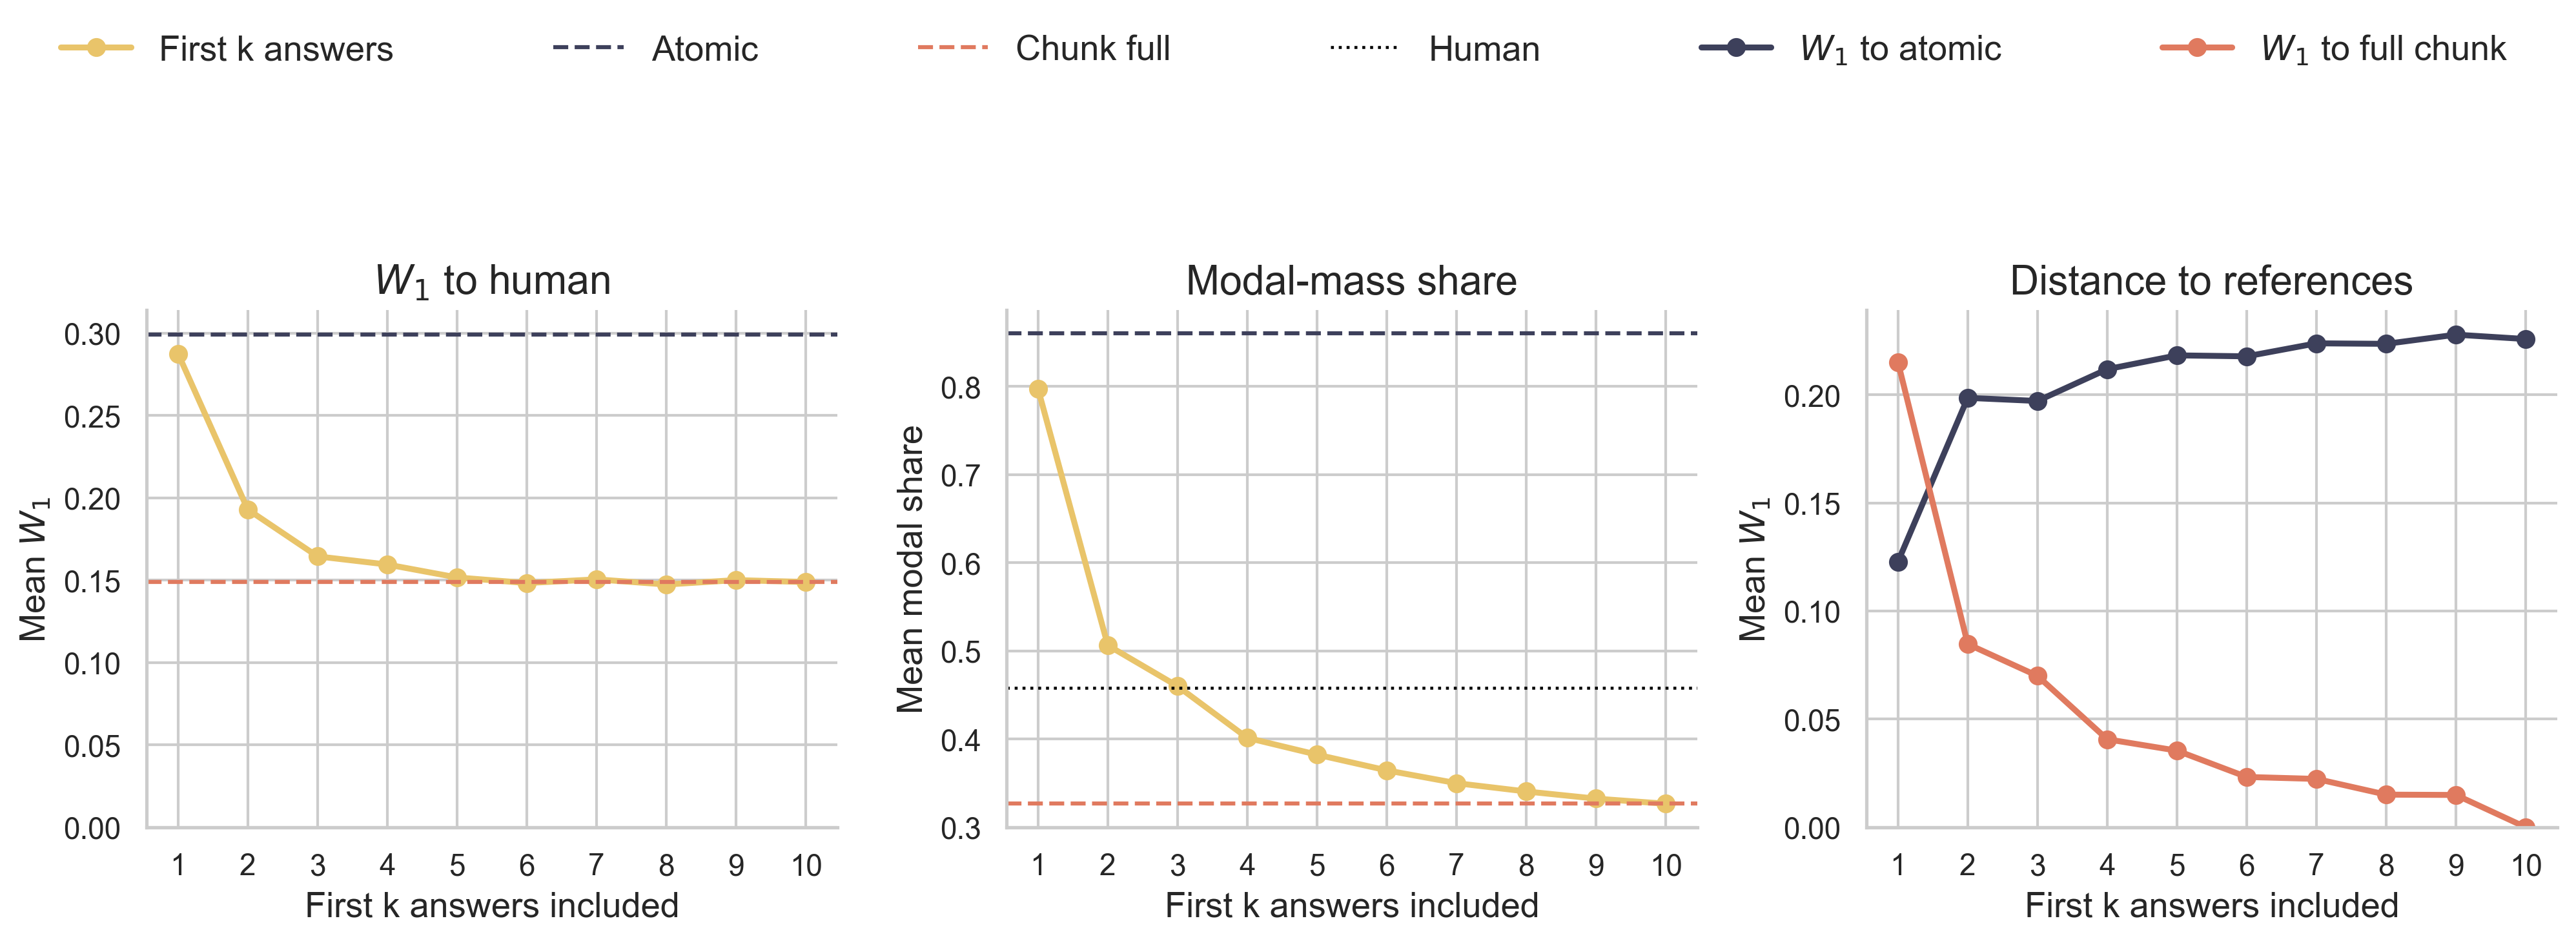
\includegraphics[width=\textwidth]{mechanism_cumulative_answer_w1.png}
\caption{Distance and concentration as answer positions are pooled cumulatively.}
\label{fig:mech-cumulative-answer}
\end{figure}

\end{document}
